\subsection{Introducción}
\label{section:introduction-sprint-3}
A partir de este Sprint, se comenzará a implementar la integración con Scopus y toda lógica relacionada con el servidor. 

Para este Sprint específico, se establecerá el ambiente de desarrollo con las herramientas necesarias para la implementación.
Además, se rediseñará la base de datos orientada a grafos utilizando Neo4j, Django y Neomodel como ORM, basándonos en el diseño en Neo4j propuesto en Resnet.
Se trabajará en la implementación de los modelos en Neomodel.

Finalmente, se pretende exponer el uso de Arquitectura Hexagonal para la implementación de la funcionalidad de búsqueda de autores. Cabe destacar que este será el único sprint en el que se ahondará en la Arquitectura Hexagonal;
los demás sprints no tendrán ese nivel de detalle.

\subsection{Objetivos}

\begin{itemize}
    \item Levantar el ambiente de desarrollo
    \item Implementar y rediseñar los modelos de la base de datos en Neo4j a través de Neomodel.
    \item Desarrollar la funcionalidad de busqueda de autores.
\end{itemize}

\subsection{Planificación}

Para este sprint se ha seleccionado las historias de usuario que se muestran en la tabla \ref{C2T3:Historias de Usuario del Sprint 3}.

\begin{table}[H]
    \centering
    \begin{tabular}{|p{2.5cm}|p{5cm}|p{6cm}|}
        \midrule
        \textbf{Identificador} & \textbf{Historia de Usuario}                                                                                                                                                                               & \textbf{Tareas} \\
        \hline
        HU-SE-02 & Como usuario no registrado deseo poder ver los investigadores que tengan colaboraciones en artículos con afiliaciones ecuatorianas para mantenerme informado sobre sus investigaciones y campos de estudio &
        \begin{compactitem}
            \item Crear servicios para el modelo de autor
            \item Diseñar el endpoint que maneje las solicitudes del autor
        \end{compactitem}
        \\
        \hline
        HU-SE-05 & Como desarrollador de software, quiero migrar nuestro modelo de base de datos actual a Neomodel, para que podamos aprovechar las capacidades del ORM Neomodel para simplificar la gestión de datos y mejorar la integración con nuestro proyecto Django.&
        \begin{compactitem}
            \item Definir los modelos, relaciones y propiedades de los nodos.
            \item Hacer las migraciones desde Django a Neo4j.
        \end{compactitem}
        \\
        \hline
        HU-SE-06 & Como desarrollador, quiero configurar un entorno de desarrollo replicable, para asegurar que podamos contar con un entorno completamente aislado y consistente que optimice el flujo de trabajo&
        \begin{compactitem}
            \item Crear el contenedor de Docker para al aplicación de backend
            \item Crear  un orquestador de contenedores
            \item Orquestar los servicios de la aplicación y la base de datos
        \end{compactitem}
        \\
        \hline
    \end{tabular}
    \caption{Historias de Usuario del sprint 3}
    \label{C2T3:Historias de Usuario del Sprint 3}
\end{table}


A continuación en las Figuras \ref{fig:aceptance-criteria-HU-SE-02}, \ref{fig:aceptance-criteria-HU-SE-05} y \ref{fig:aceptance-criteria-HU-SE-06}
se muestran los criterios de aceptación para las historias de usuario seleccionadas.
\begin{figure}[H]
    \centering
    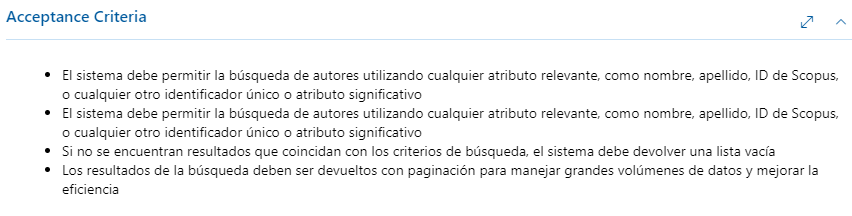
\includegraphics[scale=0.7]{../02Figures/02Chapter/Sprints/Sprint-3/aceptance-criteria-HU-SE-02.png}
    \caption{Criterios de aceptación HU-SE-02}
    \label{fig:aceptance-criteria-HU-SE-02}
\end{figure}

\begin{figure}[H]
    \centering
    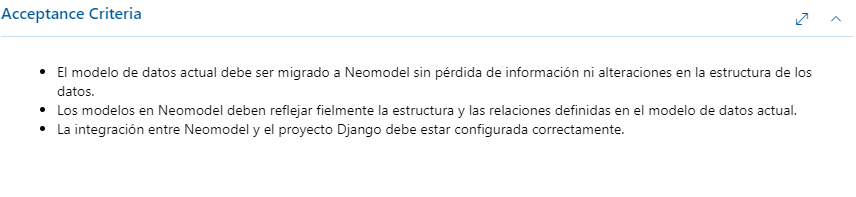
\includegraphics[scale=0.7]{../02Figures/02Chapter/Sprints/Sprint-3/aceptance-criteria-HU-SE-05.png}
    \caption{Criterios de aceptación HU-SE-05}
    \label{fig:aceptance-criteria-HU-SE-05}
\end{figure}

\begin{figure}[H]
    \centering
    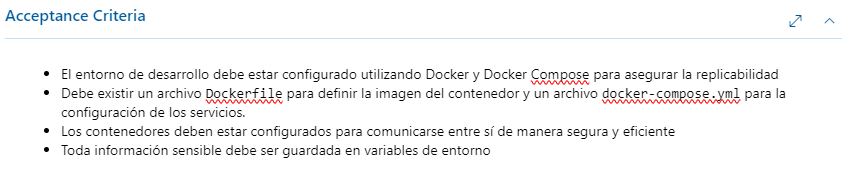
\includegraphics[scale=0.7]{../02Figures/02Chapter/Sprints/Sprint-3/aceptance-criteria-HU-SE-06.png}
    \caption{Criterios de aceptación HU-SE-06}
    \label{fig:aceptance-criteria-HU-SE-06}
\end{figure}

\subsection{Implementación}
Para el desarrollo del Sprint 3 se empezó con la configuración del entorno de desarrollo, se utilizó Docker para la creación de contenedores y Docker Compose para la orquestación de los servicios.
Para dockerizar la aplicación se creó un archivo Dockerfile en la raíz del proyecto, en el cual se especifican las instrucciones necesarias para la creación de la imagen de la aplicación, tal como se muestra Figura \ref{fig:dockerfile}.

\begin{figure}[!t]
    \centering
    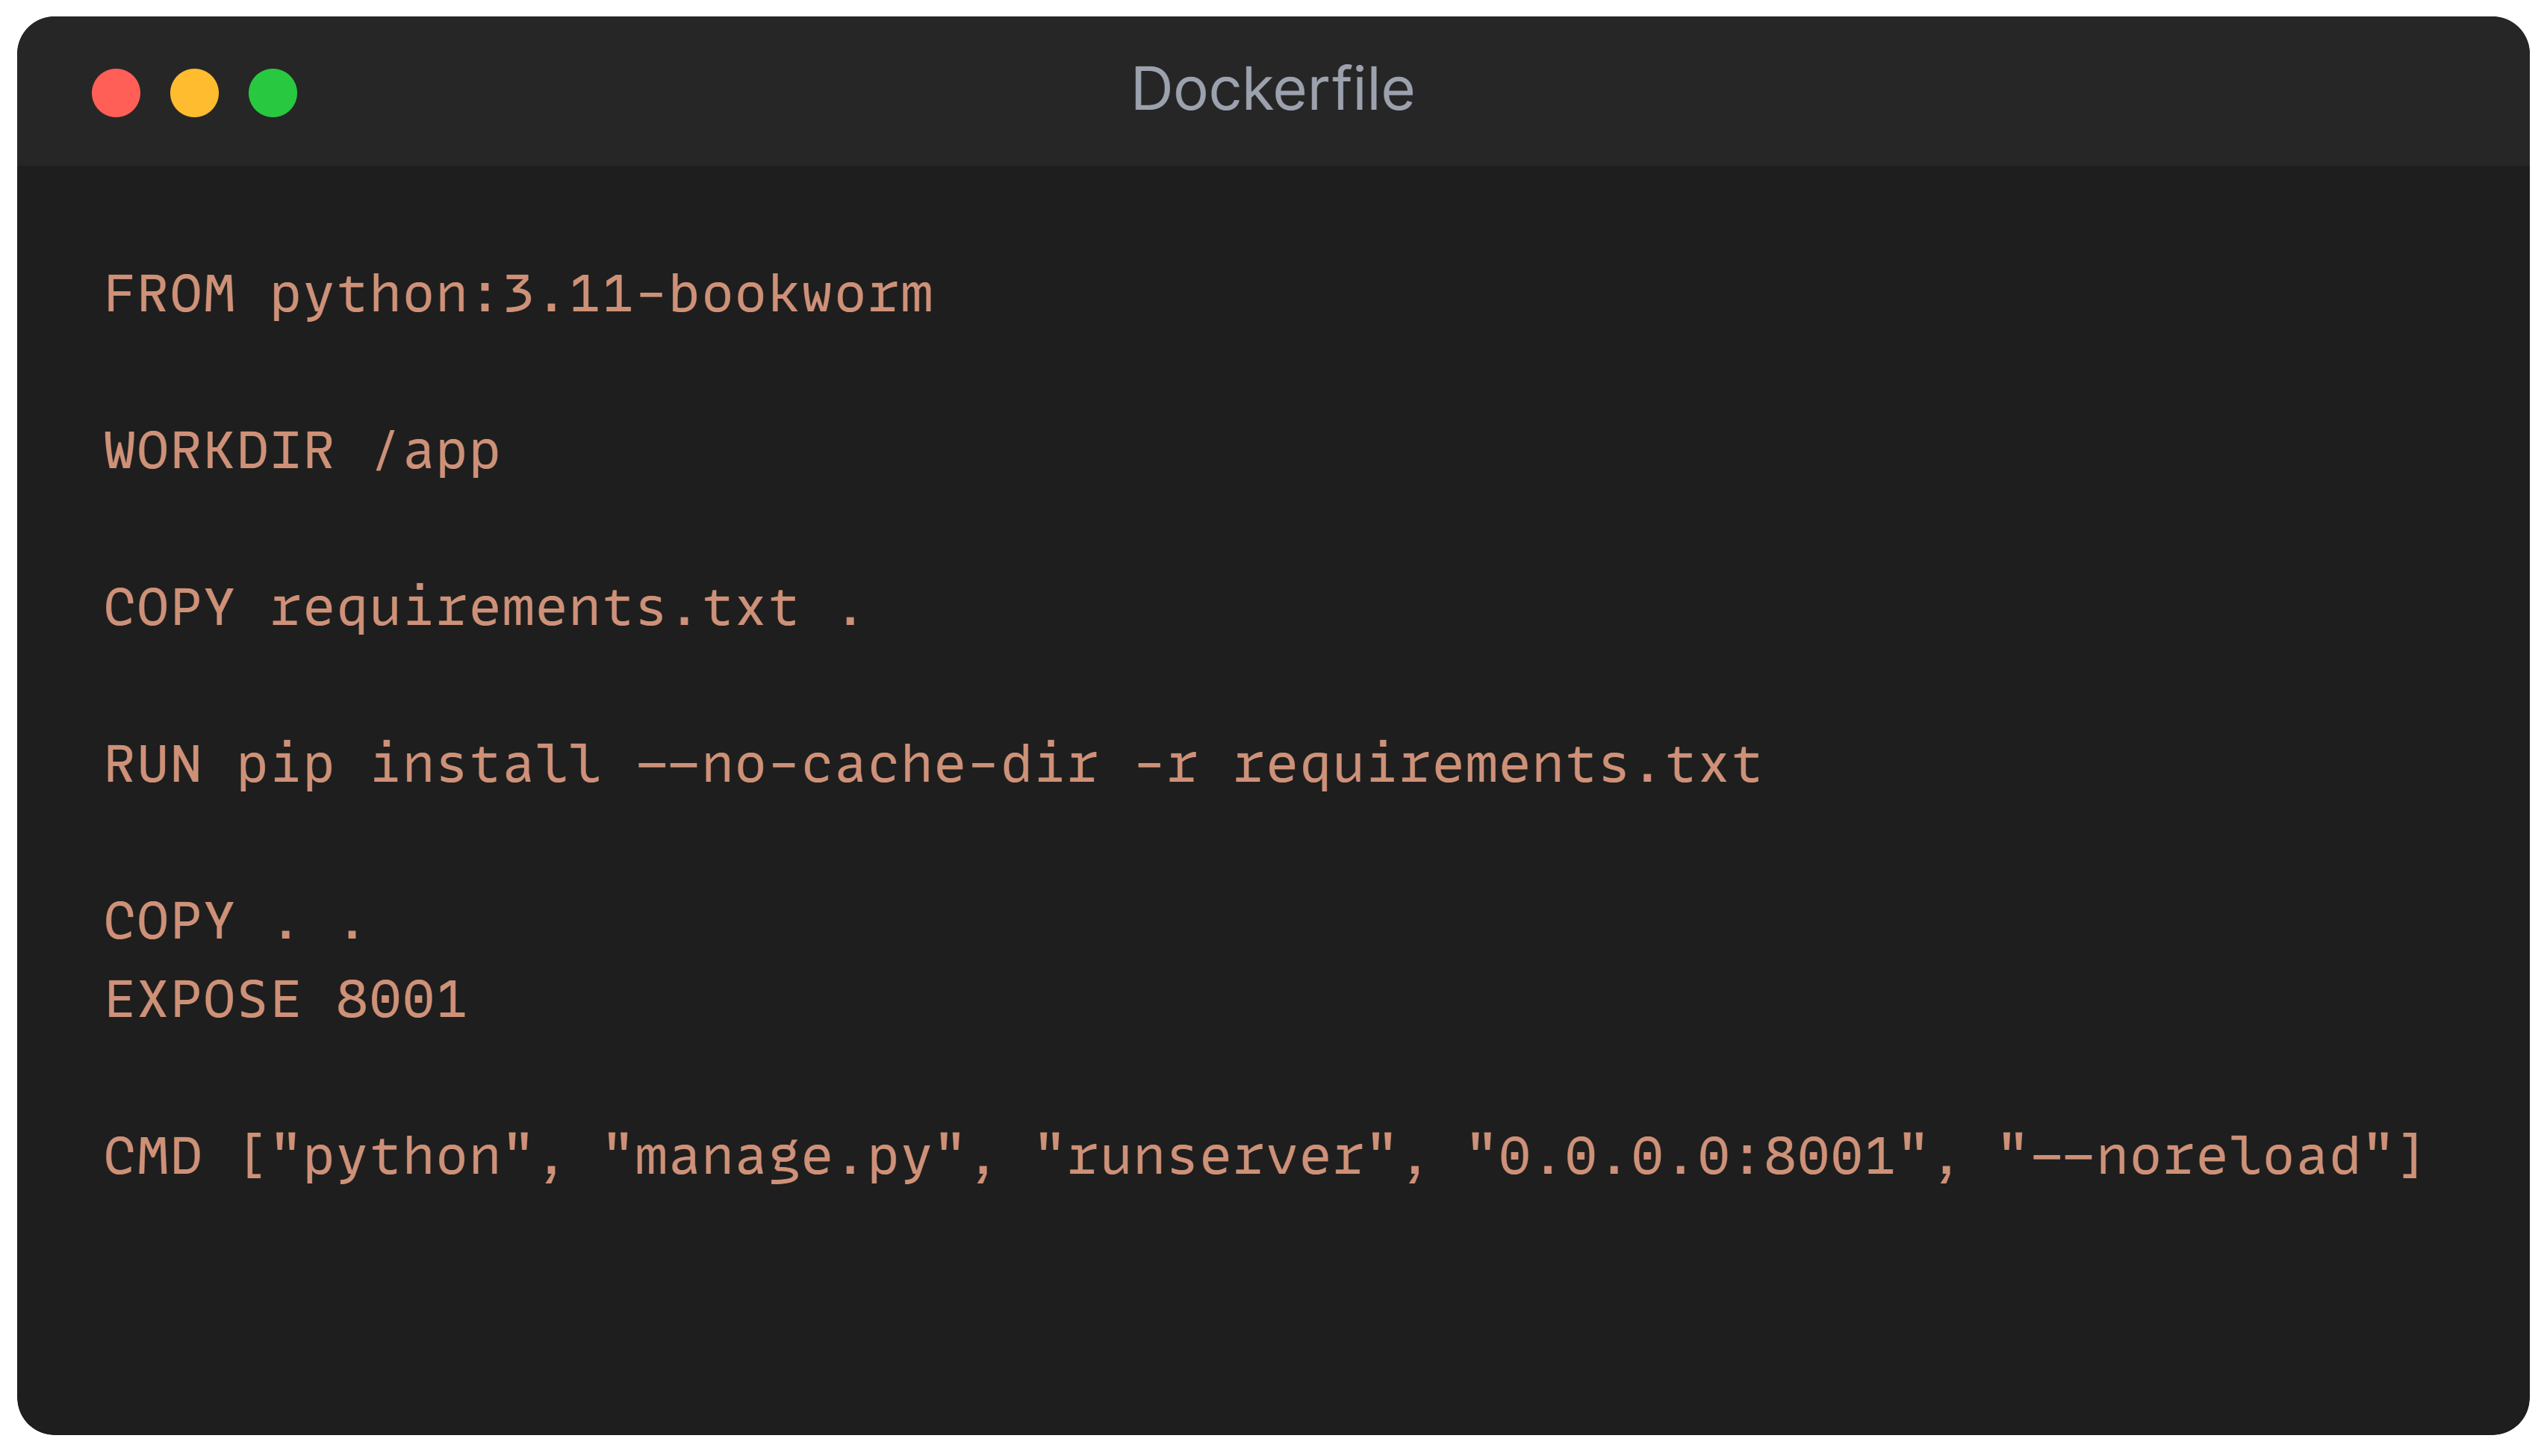
\includegraphics[scale=0.12]{../02Figures/02Chapter/Sprints/Sprint-3/Dockerfile.png}
    \caption{Archivo Dockerfile}
    \label{fig:dockerfile}
\end{figure}

En la Figura \ref{fig:docker-compose} se muestra el archivo de configuración de Docker Compose.
El mismo se encarga de orquestar los servicios de la aplicación y la base de datos. Tambien se asegura de persistir los datos de la base de datos en un volumen de Docker.
De la misma manera se especifican las variables de entorno necesarias para la configuración y el correcto funcionamiento de la aplicación.

\begin{figure}[!t]
    \centering
    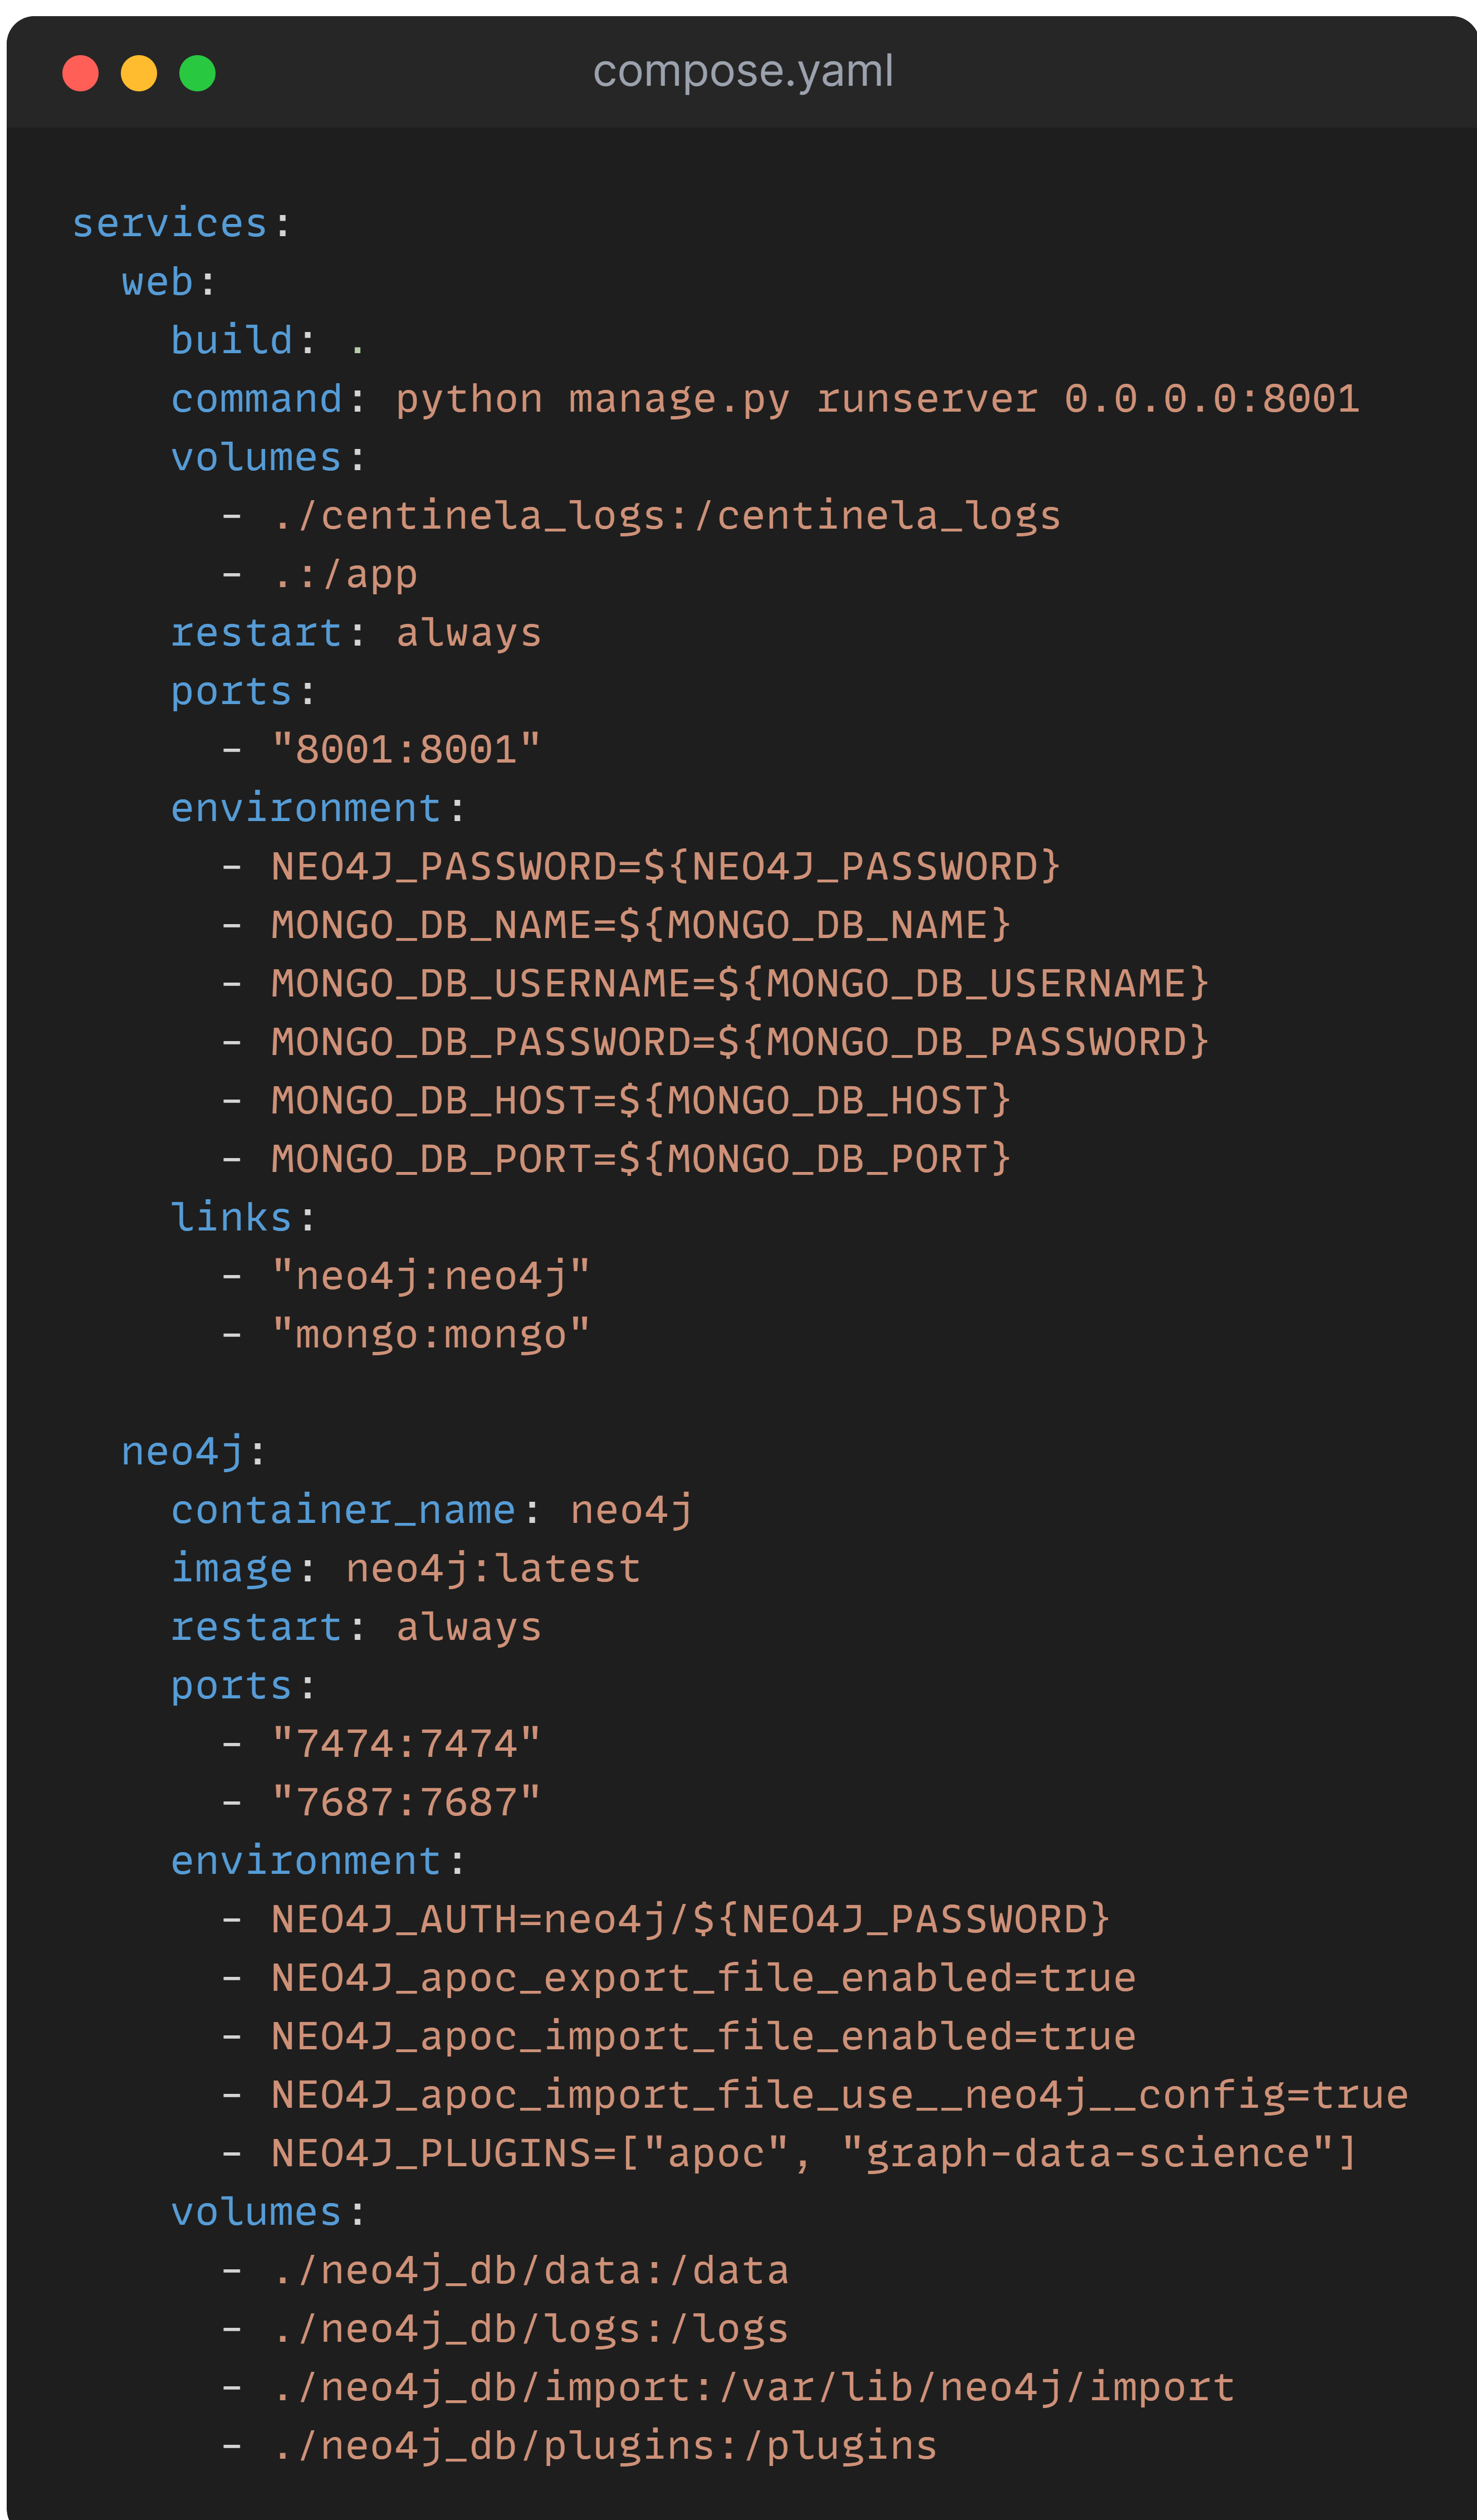
\includegraphics[scale=0.12]{../02Figures/02Chapter/Sprints/Sprint-3/compose-yaml.png}
    \caption{Archivo Docker Compose}
    \label{fig:docker-compose}
\end{figure}

Una vez configurado los archivos de Docker y Docker Compose,
se procedió a levantar los contenedores con el comando \textit{docker-compose up --build}.
Este comando se encarga de construir y levantar los servicios de la aplicación y la base de datos.
Para verificar que los contenedores se encuentran en ejecución se utiliza el comando \textit{docker ps}.
En la Figura \ref{fig:docker-ps} se muestra la salida del comando \textit{docker ps}.

\begin{figure}[H]
    \centering
    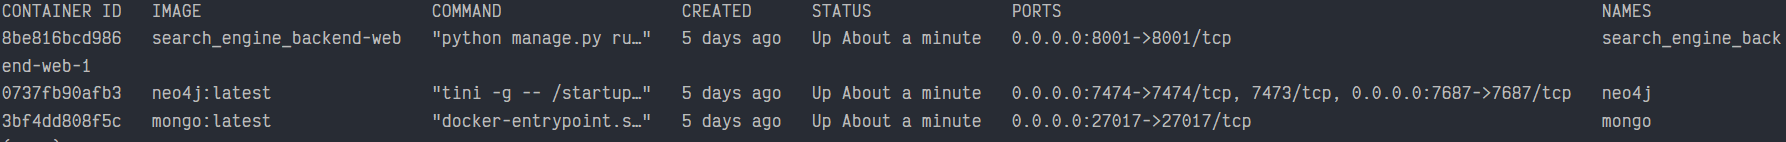
\includegraphics[scale=0.4]{../02Figures/02Chapter/Sprints/Sprint-3/docker-ps.png}
    \caption{Sialida del comando docker ps}
    \label{fig:docker-ps}
\end{figure}

Con el entorno de desarrollo configurado. Se procedió a la creación de las aplicaciones de Django.
Django denomina aplicaciones a un conjunto de funcionalidades que se pueden reutilizar en diferentes proyectos.
En este caso se crearon 3 aplicaciones \textit{dashboards}, \textit{scopus\_integration} y \textit{search\_engine}. Las mismas que se pueden observar en la Figura \ref{fig:django-apps}.
\begin{figure}[H]
    \centering
    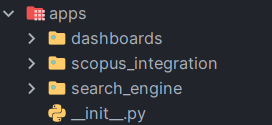
\includegraphics[scale=1]{../02Figures/02Chapter/Sprints/Sprint-3/django-apps.png}
    \caption{Aplicaciones de Django}
    \label{fig:django-apps}
\end{figure}

Las mismas que tendrán la estructura de carpetas en base a Arquitectura Hexagonal, como se menciono en la Seccion \ref{chapter02-section02-sprint0}.
Cada aplicación tendrá su propia capa de dominio, aplicación e infraestructura.
Así como cada una tendra una función específica en la aplicación, \textit{dashboards} se encargara de la visualización de los datos, \textit{scopus\_integration} de la integración con Scopus y \textit{search\_engine} de la funcionalidad del motor de busqueda.

Una vez finalizada la creación de las aplicaciones,  procedió a hacer el rediseño de la base de datos
previo a la implementación de los modelos en Neonmodel. Como se menciono en la Seccion \ref{section:introduction-sprint-3} se tomo como base el diseño en Neo4j propuesto en Resnet.
Unicamente se agrego nuevos atributos a los nodos y relacione existentes.
Mas especificamente se agregaron atributos al nodo de \textit{Autor} y a la relación \textit{COAUTHORED}.
En la Figura \ref{fig:neo4j-model} se muestra el diseño de la base de datos.

\begin{figure}[H]
    \centering
    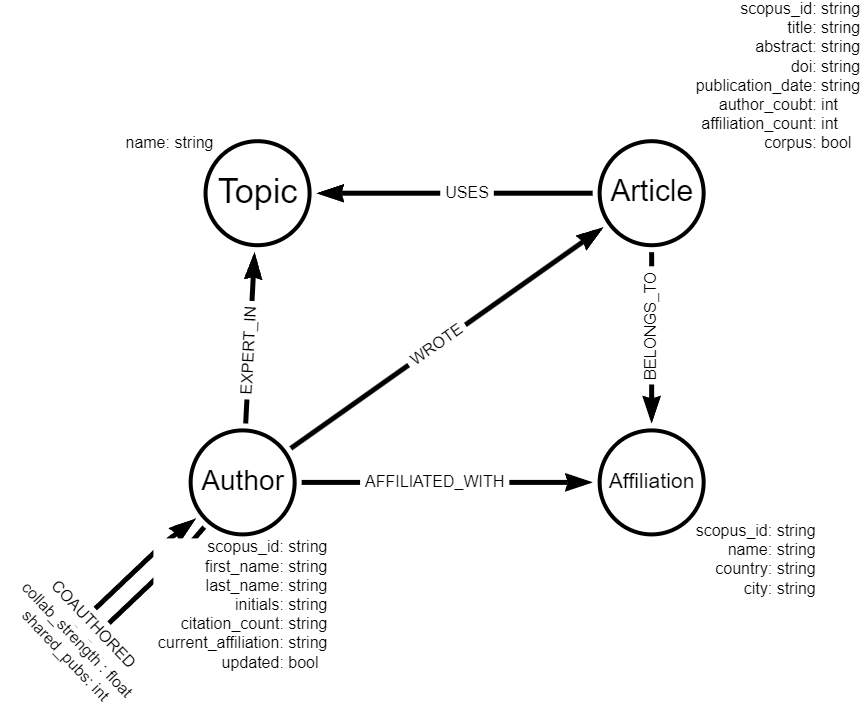
\includegraphics[scale=0.5]{../02Figures/02Chapter/Sprints/Sprint-3/centinela-graph.design-light.png}
    \caption{Modelo de la base de datos }
    \label{fig:neo4j-model}
\end{figure}

Con estas actualizaciones en el modelo, se procedió a la implementación de los mismos en Neomodel.
Como se menciono en el Sprint 0, para el desarrollo de la aplicación
se utilizara Arquitectura Hexagonal. Bajo este enfoque se crearon los modelos de la base de datos en la capa de dominio.
En la Figura \ref{fig:domain-layer} se muestra la capa de dominio de la aplicación que se encargara del motor de busqueda.

\begin{figure}[H]
    \centering
    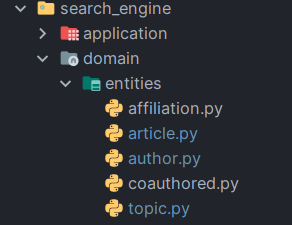
\includegraphics[scale=0.9]{../02Figures/02Chapter/Sprints/Sprint-3/domain-layer.png}
    \caption{Capa de dominio de la aplicación}
    \label{fig:domain-layer}
\end{figure}

Basandonos en el diseño de la base de datos que se muestra en la Figura \ref{fig:neo4j-model},
se muestra el modelo \textit{Author} implementado con Neomodel en la Figura \ref{fig:author-model}.
En terminos generales para asegurar la integridad de los datos se hace uso  de las restricciones de unicidad de Neomodel, con el tipo de dato \textit{UniqueIdProperty}.
Esto será de gran utilidad para evitar la creación de nodos duplicados en la base de datos.
Asimismo se utilizan las propiedades de tipo \textit{Relationship} y \textit{RelationshipTo} para definir las relaciones entre los nodos.

\begin{figure}[H]
    \centering
    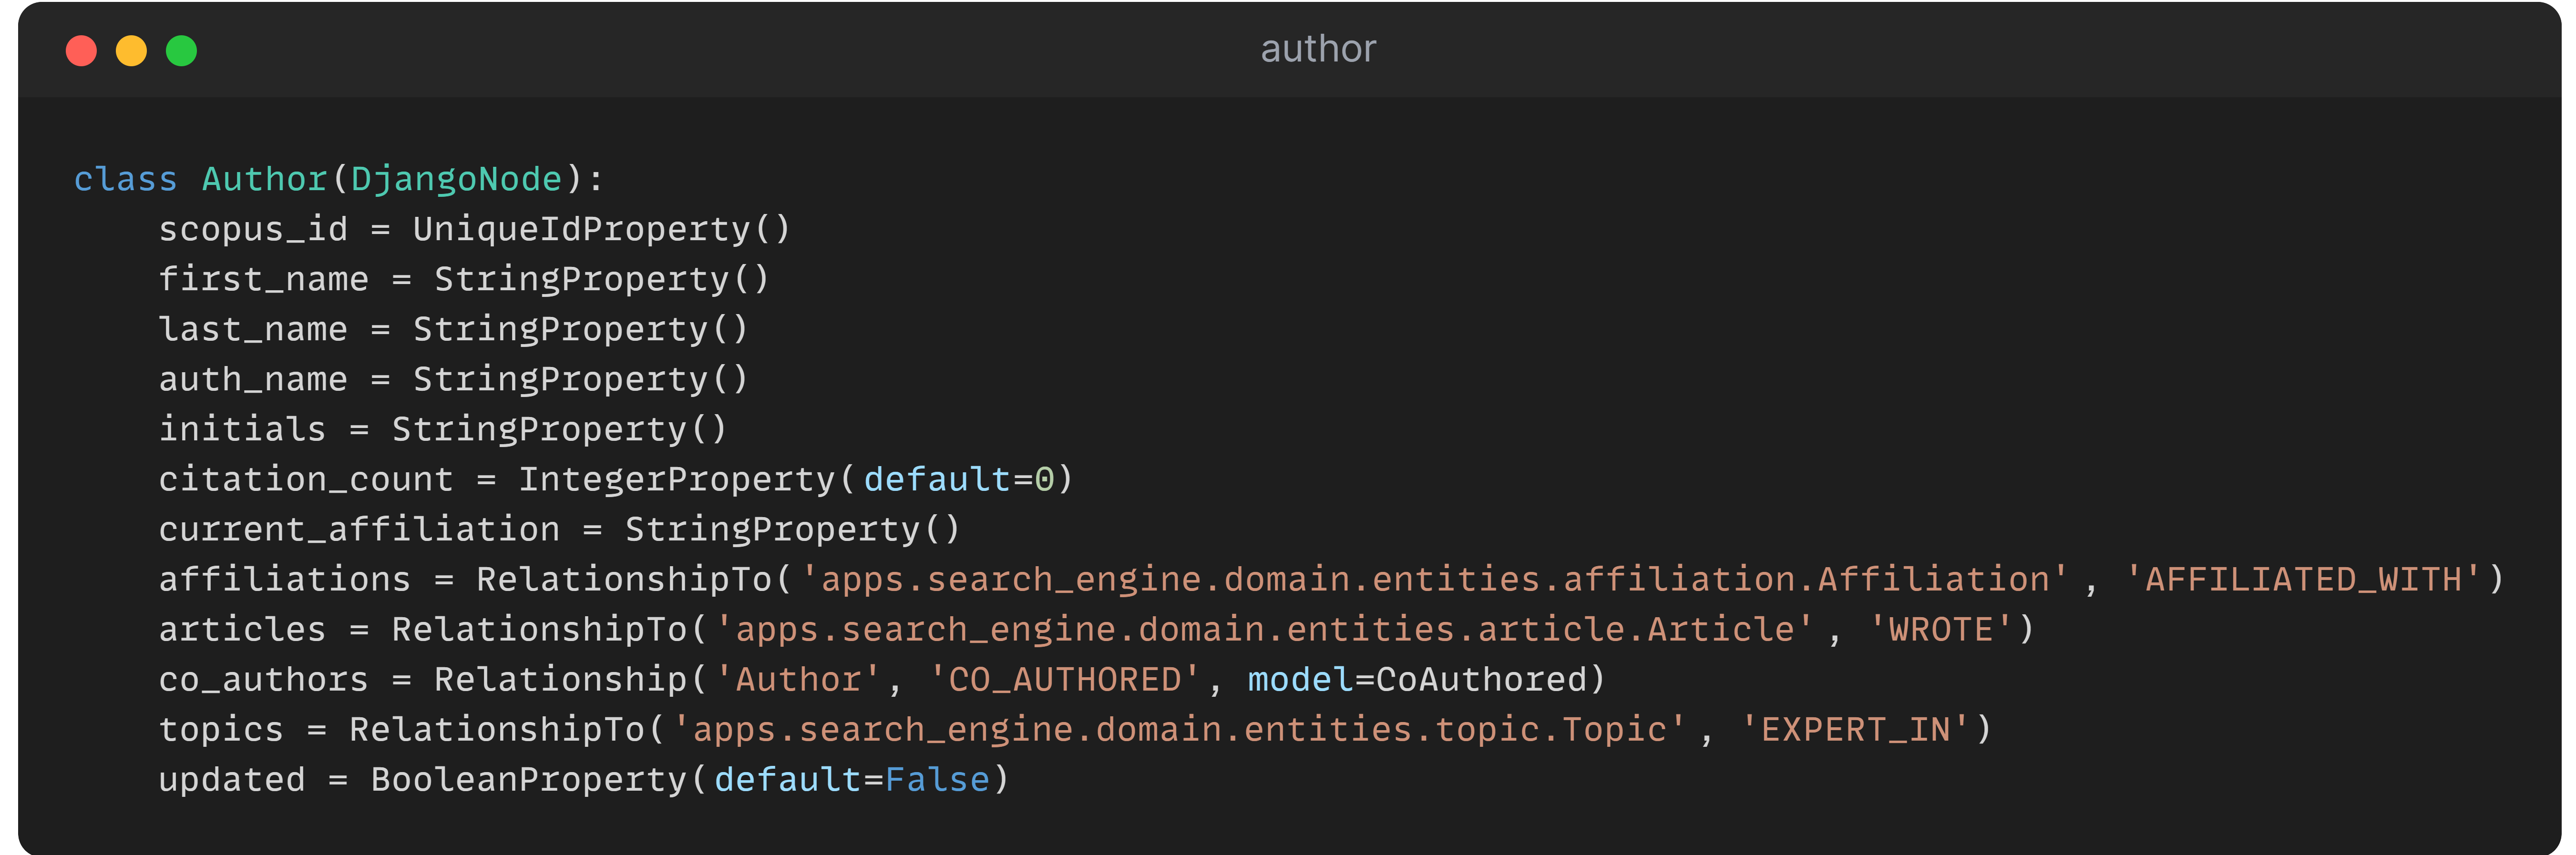
\includegraphics[scale=0.12]{../02Figures/02Chapter/Sprints/Sprint-3/author-neomodel.png}
    \caption{Modelo Author implementado con Neomodel}
    \label{fig:author-model}
\end{figure}

Finalmente la migración de estos modelos a la base de datos se realiza con el comando \texttt{python manage.py install\_labels}.
Aunque este comando es opcional es recomendable ejecutarlo para asegurar que los modelos se encuentren en la base de datos, o si en su defecto se requiere hacer una actualización de los modelos.

Siguiendo la Arquitectura Hexagonal, se procedió a implementar la funcionalidad de búsqueda de autores.
Para ello, se creó el repositorio AuthorRepository en la capa de dominio, encargado de definir los métodos necesarios para la búsqueda de autores.

El uso del patrón de diseño Repository garantiza la separación entre la lógica de negocio y la lógica de persistencia. Posteriormente, en la capa de aplicación, se implementará la lógica de negocio correspondiente a cada una de las funciones definidas en el repositorio.

En la Figura \ref{fig:author-repository} se muestra un extracto del repositorio \textit{AuthorRepository} con algunos de los métodos que nos serviran para la busqueda de autores.

\begin{figure}[H]
    \centering
    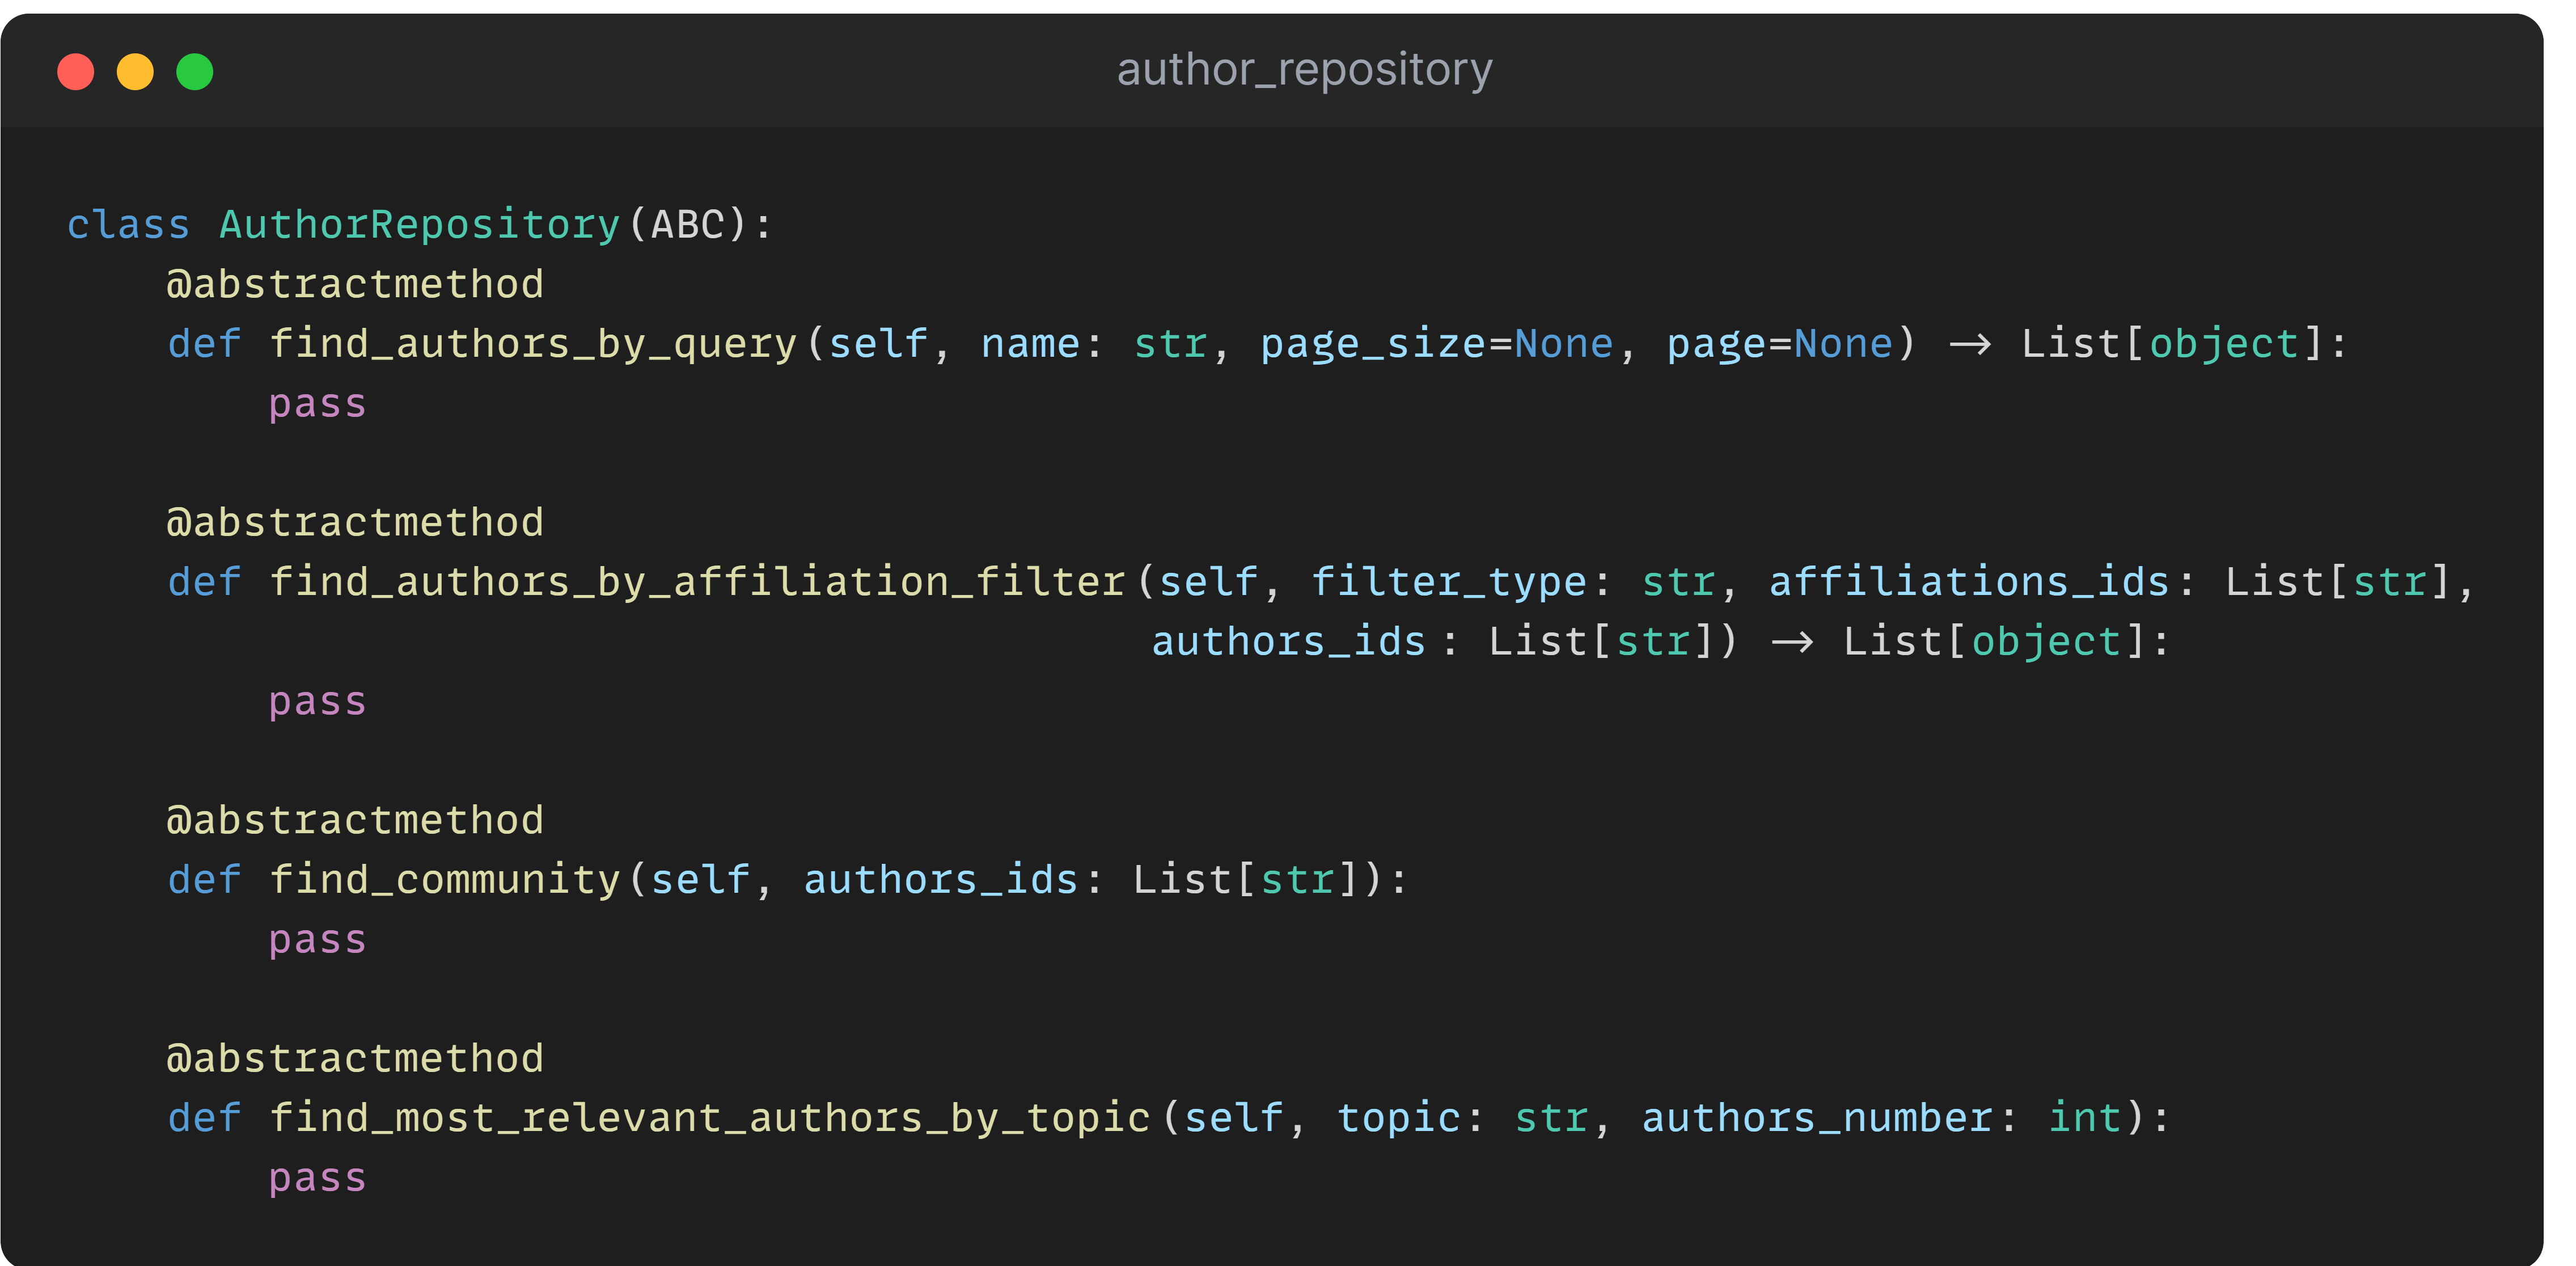
\includegraphics[scale=0.13]{../02Figures/02Chapter/Sprints/Sprint-3/author-repository.png}
    \caption{Repositorio AuthorRepository}
    \label{fig:author-repository}
\end{figure}

Una vez definidos los repositorios pasamos a la capa de aplicación, en la cual se implementa la lógica de negocio correspondiente a cada uno de los métodos definidos en el repositorio.
La Figura \ref{fig:author-service} muestra un extracto del servicio \textit{AuthorService} el mismo que hereda de la clase \textit{AuthorRepository} con la implementación de la función \textit{find\_authors\_by\_query}.

\begin{figure}[H]
    \centering
    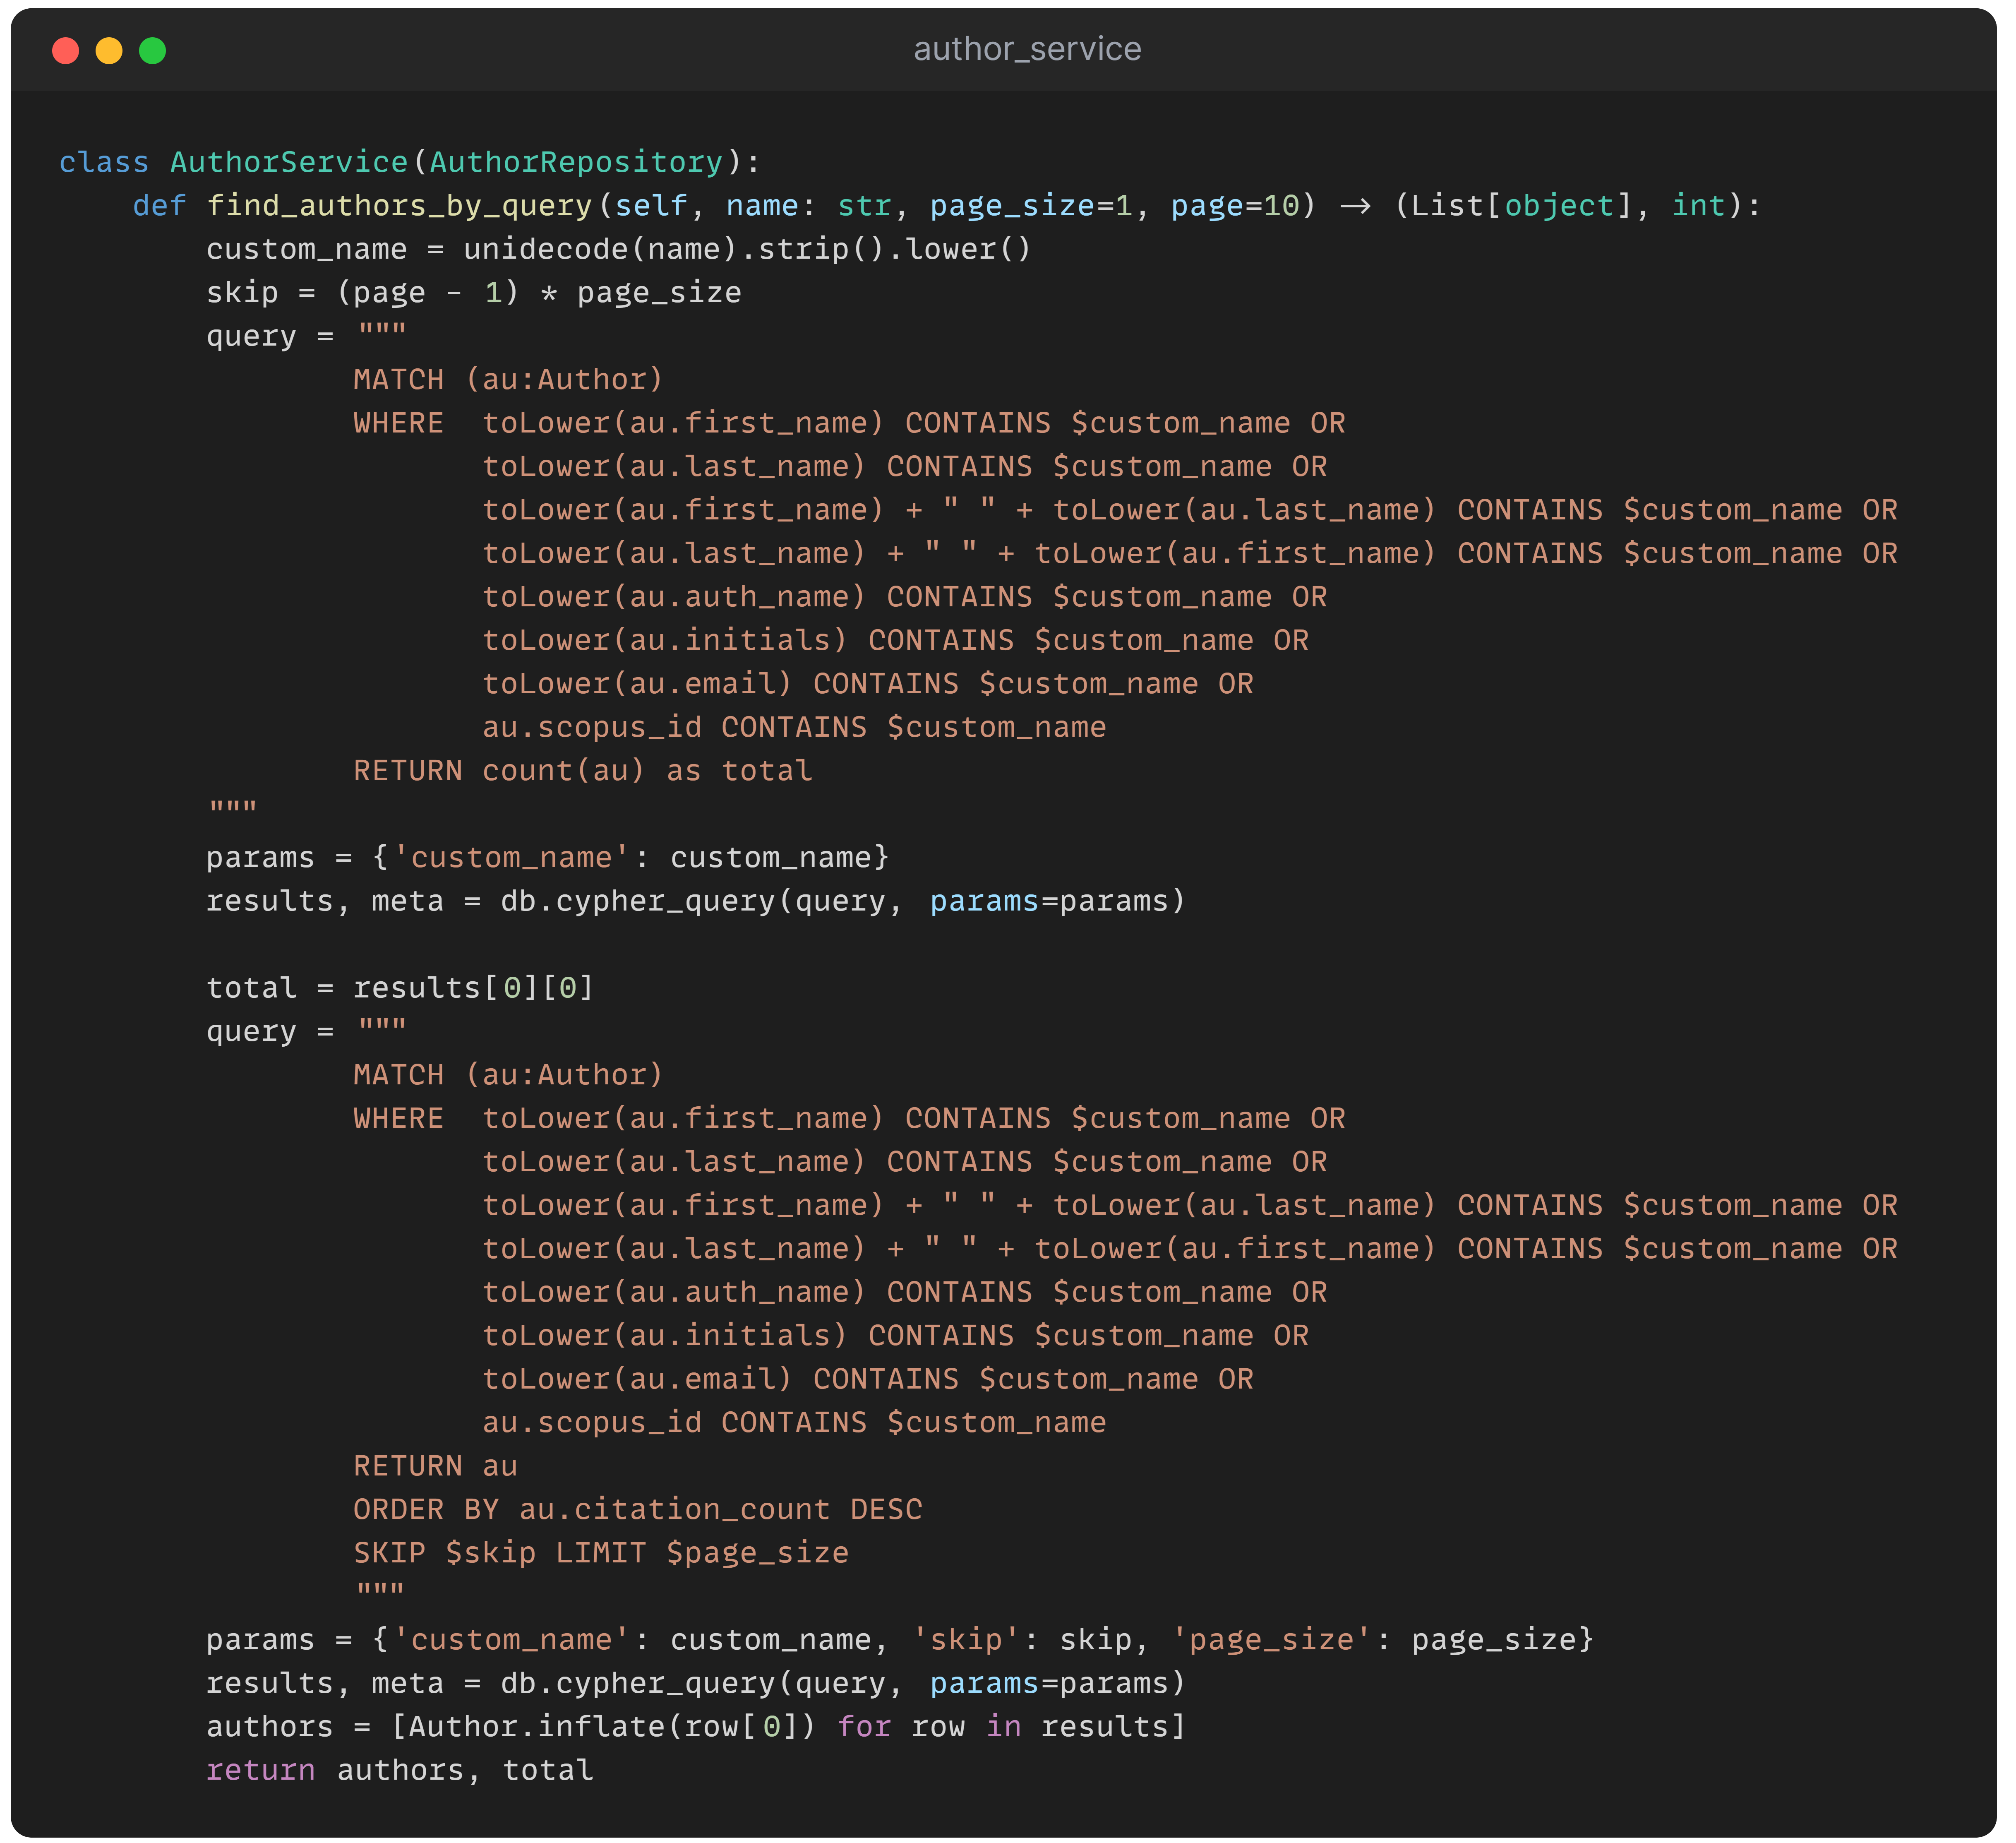
\includegraphics[scale=0.11]{../02Figures/02Chapter/Sprints/Sprint-3/author-service.png}
    \caption{Servicio AuthorService}
    \label{fig:author-service}
\end{figure}


Dado que en este caso se está utilizando una base de datos orientada a grafos,
se empleó el lenguaje de consulta Cypher para realizar la búsqueda de autores.
Usar Cypher permite aprovechar las ventajas de las bases de datos orientadas a grafos,
como la rapidez en la consulta de datos y la facilidad para encontrar relaciones entre los nodos.

Sin embargo, existe el riesgo de Cypher Injection, por lo que es fundamental tener
cuidado al construir las consultas. Para todas las consultas,
se utilizó el método \textit{cypher\_query} de Neomodel, que permite ejecutar consultas Cypher directamente en la base de datos,
enviando los parámetros no en la cadena de texto sino como argumentos de la función.
Esto evita la inyección de Cypher en la base de datos,
sanitizando las consultas y protegiéndolas de posibles inyecciones de Cypher.

Una vez con el servicio listo se procedió a la implementación del caso de uso \textit{FindAuthorsByQuery} en la capa de aplicación.
En la Figura \ref{fig:find-authors-by-query} se muestra el caso de uso que se encargara de llamar a los repositorios necesarios para la busqueda de autores.

\begin{figure}[H]
    \centering
    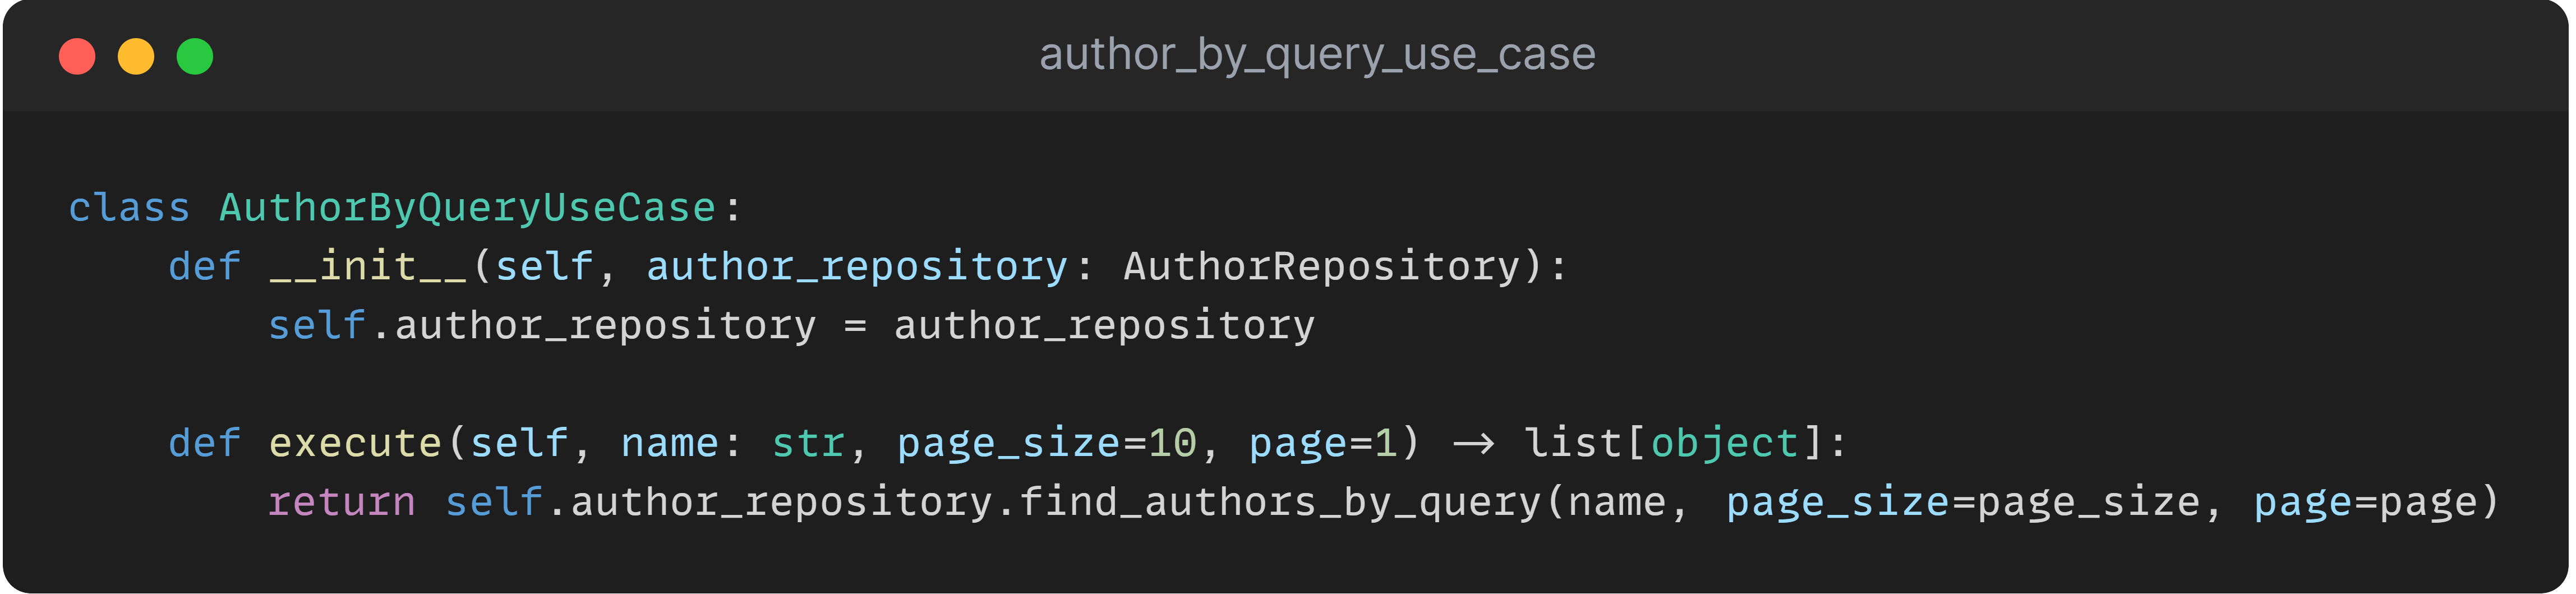
\includegraphics[scale=0.11]{../02Figures/02Chapter/Sprints/Sprint-3/author-by-query-use-case.png}
    \caption{Caso de uso FindAuthorsByQuery}
    \label{fig:find-authors-by-query}
\end{figure}

A continuación se procedió a la implementación de la capa de infraestructura.
Esta capa se va a encargar de la comunicación con el exterior de la aplicación, en este caso con la API REST.
Para ello se creó la vista \textit{AuthorViews} que se encargará de recibir las peticiones HTTP y llamar a los casos de uso correspondientes.
En la Figura \ref{fig:author-views} se muestra un extracto de la vista \textit{AuthorViews} con la implementación del caso de uso \textit{FindAuthorsByQuery}.
Como se puede observar, la vista unicamente se encarga de recibir la petición HTTP y llamar al caso de uso correspondiente. No maneja la lógica de negocio.
Esto permite que la vista sea independiente de la lógica de negocio y de la lógica de persistencia. De esta manera, se garantiza la separación de responsabilidades y se facilita la reutilización de código, logrando que la aplicación sea más mantenible y escalable.
\begin{figure}[H]
    \centering
    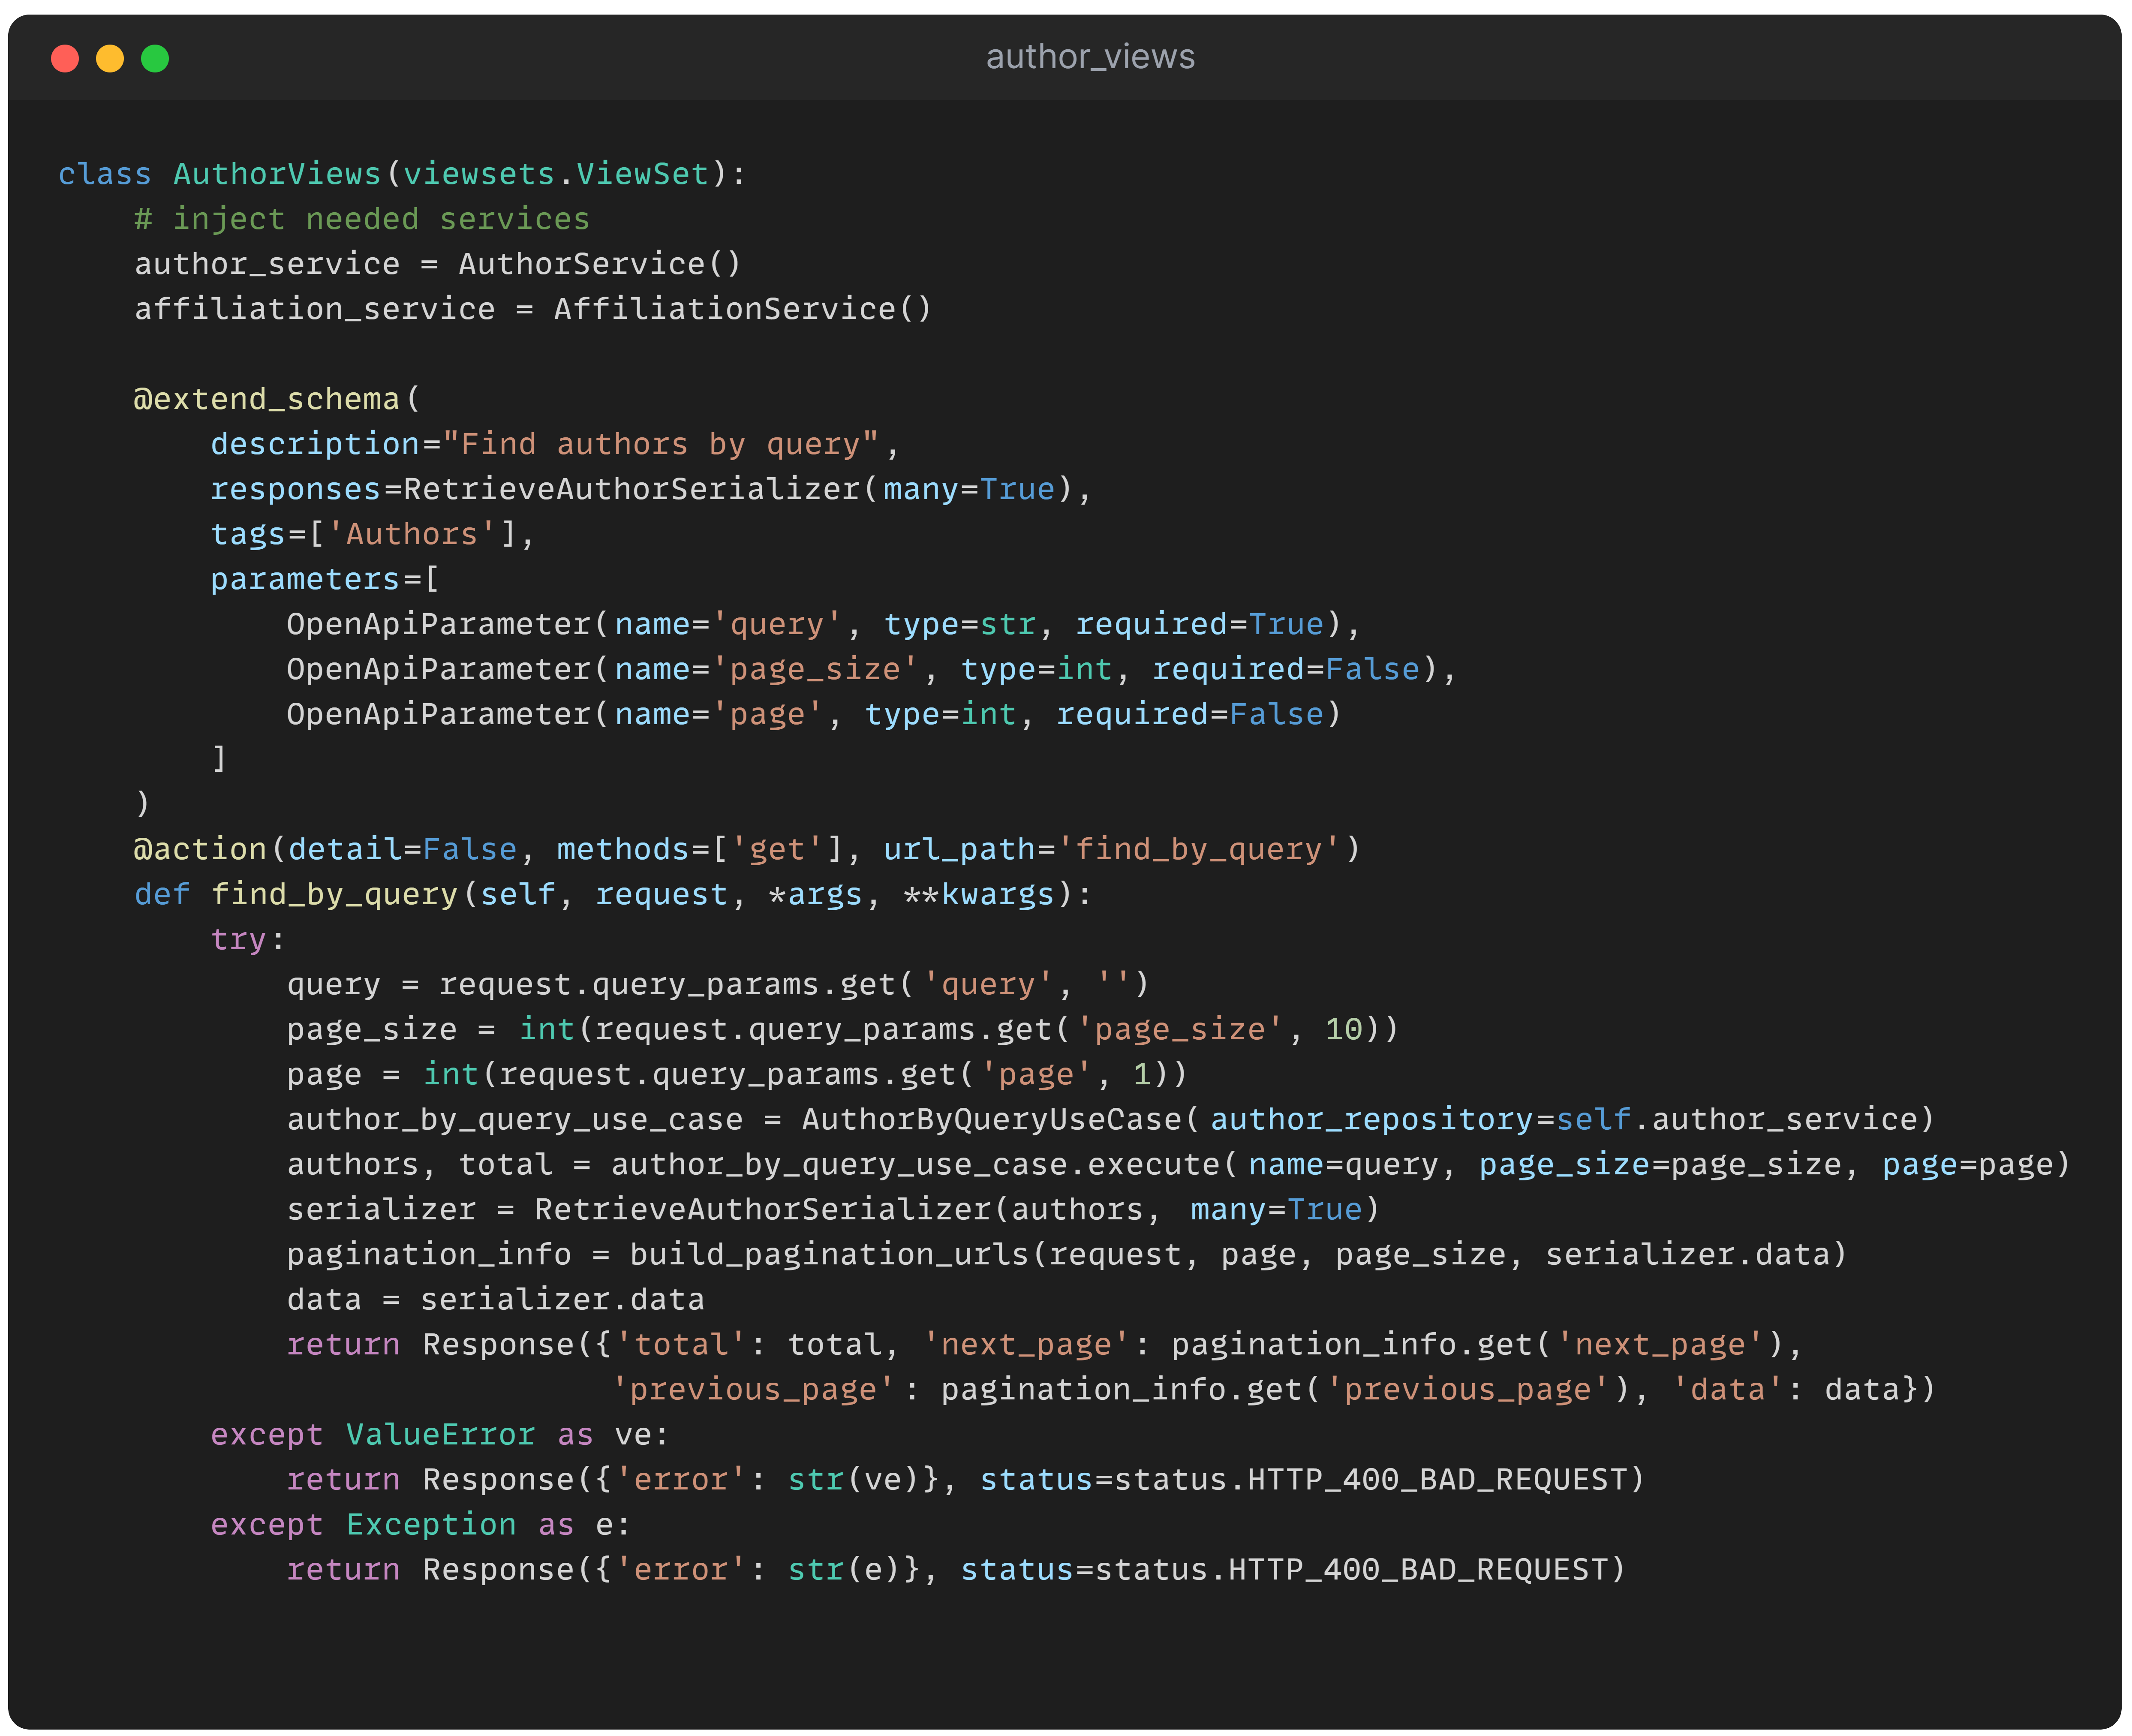
\includegraphics[scale=0.085]{../02Figures/02Chapter/Sprints/Sprint-3/author-views.png}
    \caption{Vista AuthorViews}
    \label{fig:author-views}
\end{figure}

Tambien se implemento la serialización de los datos en la capa de infraestructura.
Para ello se creo el serializador \textit{AuthorSerializer} que se encargara de serializar los datos de los autores.
Ademas, se utilizo Swagger para documentar la API REST. En la Figura \ref{fig:author-views} se puede vizualizar el decorador \footnote{
    Un decorador es una función que toma otra función y extiende su funcionalidad sin modificarla.} \textit{extend\_schema} que permite la documentación automatica de la API, en este caso se documenta el endpoint \textit{find\_by\_query}.
El resultado de la documentación se muestra en la Figura \ref{fig:swagger}. La cual tiene una interfaz gráfica que permite probar los endpoints de la API.

\begin{figure}[H]
    \centering
    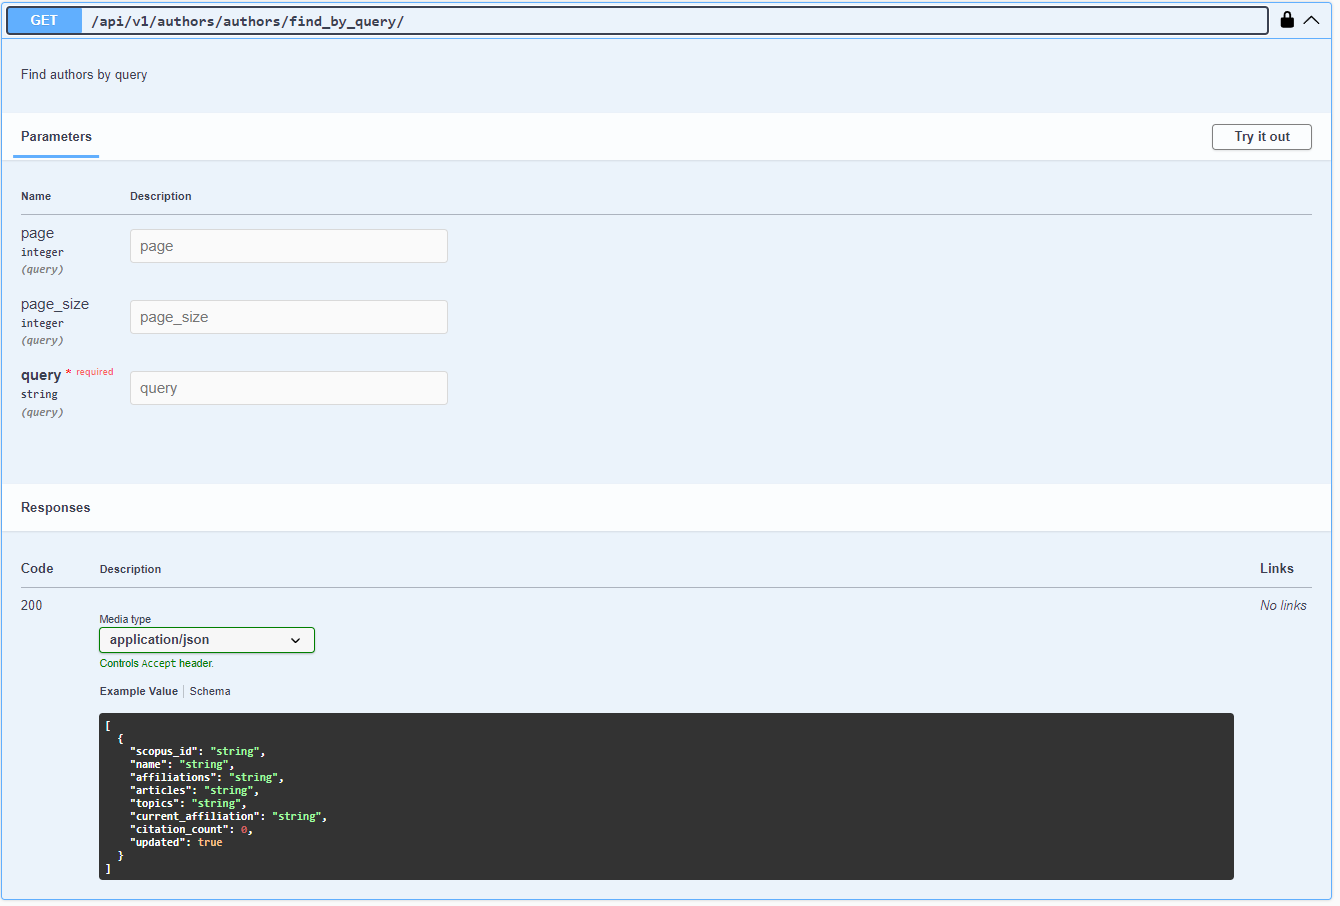
\includegraphics[scale=0.5]{../02Figures/02Chapter/Sprints/Sprint-3/swagger-ui.png}
    \caption{Documentación de la API con Swagger}
    \label{fig:swagger}
\end{figure}

Todo lo descrito anteriormente para la implementación de la funcionalidad de búsqueda de autores se puede resumir con un diagrama de secuencia.
En la Figura \ref{fig:sequence-diagram-authors-by-query} se muestra el diagrama de secuencia de la funcionalidad de búsqueda de autores.
En resumen con este diagrama de secuencia se puede observar el flujo de la aplicación. La petición HTTP llega a la vista \textit{AuthorViews}, la vista llama al caso de uso \textit{FindAuthorsByQuery}, el caso de uso llama al repositorio \textit{AuthorRepository} y este a su vez ejecuta la consulta en la base de datos.
A partir de este punto se representará unicamente el flujo de la aplicación, sin entrar en detalles de la implementación.
\begin{figure}[H]
    \centering
    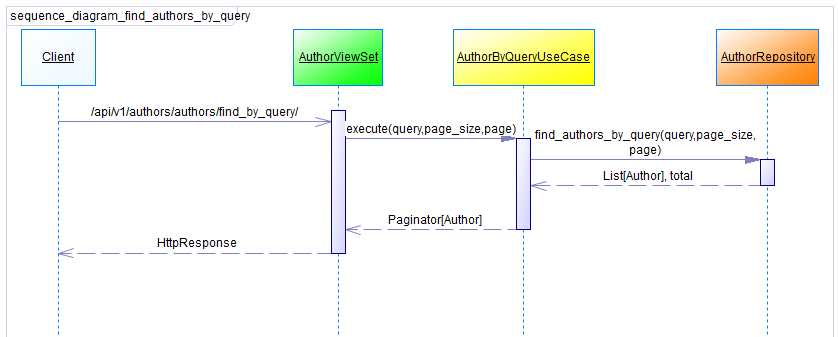
\includegraphics[scale=0.9]{../02Figures/02Chapter/Sprints/Sprint-4/sequence_diagram_find_authors_by_query.png}
    \caption{Diagrama de secuencia de la funcionalidad de búsqueda de autores}
    \label{fig:sequence-diagram-authors-by-query}
    
\end{figure}


\subsection{Revisión y Retrospectiva}
En la revision del Sprint 3 se verificó que se cumplieran los criterios de aceptación de las historias de usuario seleccionadas.
Se comprobó que la funcionalidad de búsqueda de autores funcionara correctamente y que la documentación de la API REST estuviera actualizada.
Además, se verificó que los modelos de la base de datos se encontraran en la base de datos.
En la Figura \ref{fig:neo4j-browser} se muestra la base de datos con los nodos y relaciones creados.

\begin{figure}[H]
    \centering
    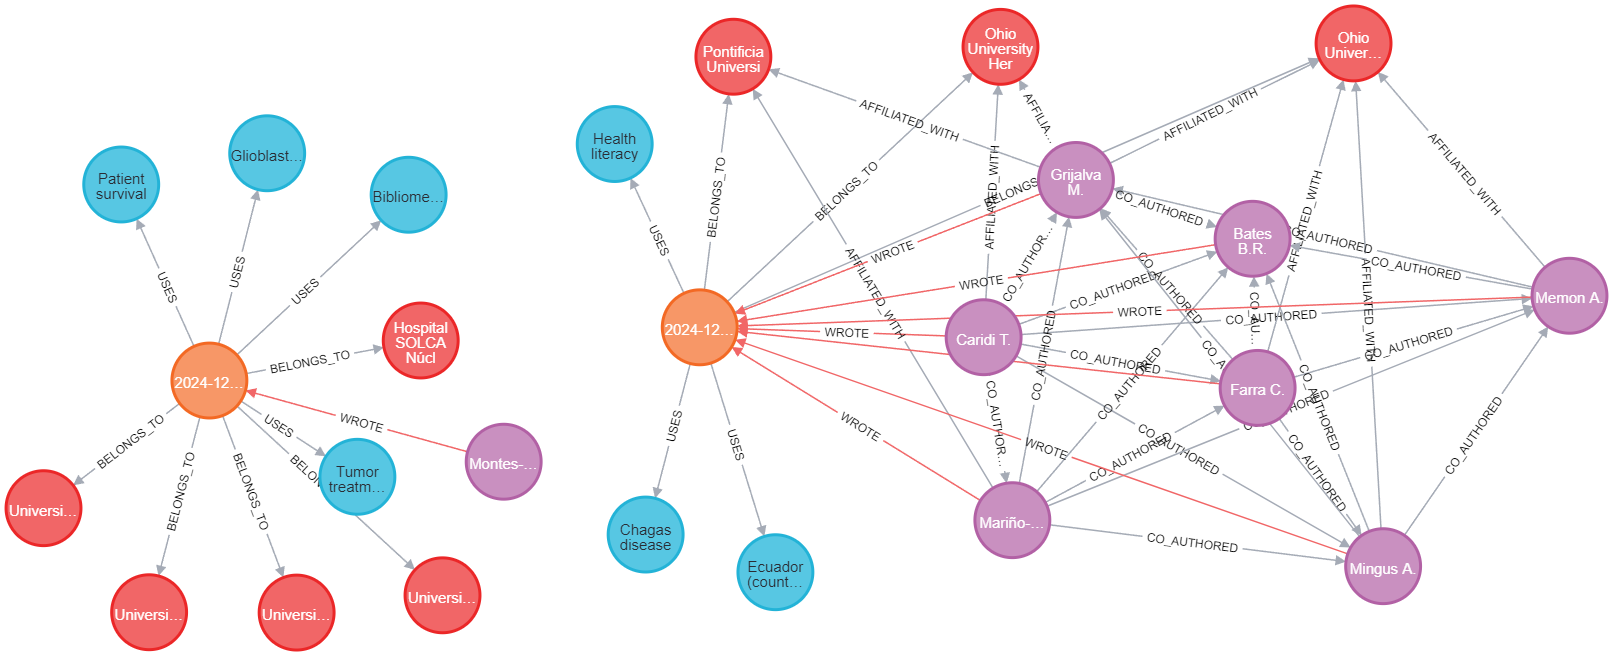
\includegraphics[scale=0.2]{../02Figures/02Chapter/Sprints/Sprint-3/graph-database.png}
    \caption{Base de datos Neo4j}
    \label{fig:neo4j-browser}
\end{figure}

Se considera que se cumplió con los objetivos planteados para este sprint, ya que se logró implementar la funcionalidad de búsqueda de autores y se rediseñó la base de datos en Neo4j utilizando Neomodel.
Además, se logró levantar el ambiente de desarrollo con Docker y Docker Compose.

Sin embargo, se presentaron algunos problemas durante el desarrollo de las tareas asignadas.
Uno de los problemas más significativos fue la falta de documentación de Neomodel, lo que dificultó la implementación de los modelos en la base de datos.
La falta de datos de prueba también fue un problema, ya que se tuvo que trabajar con datos ficticios para realizar las pruebas de la funcionalidad de búsqueda de autores.